\chapter[Studies]{Study of the existing}
Once again this part will be splitted in 2 because the subjects are totally differents. I am going to talk first about the helmet, that required 1 month of test and studies. I will explain the procedures in the next chapter. 
	
	\section{Helmet study}	
	\subsection{Helmet itself}
	\par I began my study by acquire some knowledges about the helmet itself. It has been release in the end of 2013, build for harsh condition, its price makes it unaccessible for the public. The army and building companies sow a good opportunity in this technologie to ease the work by bringing communication into the field.
	\par The helmet is equiped with a batterie, Wi-Fi and blutooth connections, a camera and it can be wear under the work helmet. Everything is voice commanded and very responsive thanks to Motorola's work. Windows CE 6.0 is used on the last release of the helmet image. It is good for the next section to understand that the booting system and the update system of windows CE are related. That means that you can change the file system for an update but it is windows itself that validate and copy the files on the intern memory from the SD card.
	\subsection{Embedded systems}
	\par I learned a lot about embbeded system, mainly on the boards and all the materials related to it. In our case, the materials inside the helmet are not know and not published on the Internet. Pierluigi contacted the company that brought us the helmet but they couldn't tell us which board was used in the helmet. I must have guessed which TI technology it was because the datasheet reference a TI OMAP 3 microprocessor. 
	\par That is mainly why I put my effort on the "ISEE – IGEP COM MODULE" built in with a TI OMAP 3 processor. It was at the top of the art when the helmet released and the smallest board with this processor. It corresponds well with the size of the hardware slot. In any case, if the linux kernel is compatible with the processor a cross compiled file system should boot and at least it should show an image on the screen.
	
	\subsection{Cross-compilation}
	\subsubsection{Description}
	\par The cross-compilation is compilation for a different achitecture than the architecture that makes the computations. In the figure~\ref{cross} you can see that the source code can be compiled for different architectures. The aim here was to compile a Linux kernel compatible with TI OMAP 3 processors from an Intel x86 machine.
	\begin{figure}[h]
		\begin{center}
			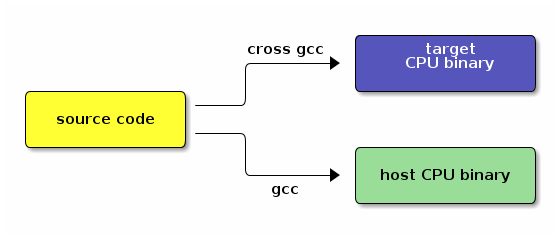
\includegraphics[scale=0.5]{images_not_compressed/cross-compile.png}
			\label{cross}
			\caption{Cross compilation and compilation difference}
		\end{center}
	\end{figure}

	\subsubsection{Process}
	\par The cross tool chain is capable of compile a Linux kernel for a lot of achitectures. Of course it requires a long time to compile the toolchain and then cross compile the kernel to get the binaries but it is cost effective. The time necessere to compile the toolchain and the kernel on the TI OMAP 3 would be longer.
	
	\subsubsection{Toolchain}
	
	\par A toolchain is a set of distinct software development tools that are linked (or chained) together by specific stages such as GCC, binutils and glibc (a portion of the GNU Toolchain)\cite{Toolchain}.
	\par A toolchain requires binutils such as assembler and linker, that produces the binaries. Also compilers for deferent languages like C, C++, Java etc, that transforms any language into another. A C library to gain access to kernel calls and a debugger that can be used or not during the compilation. We can see well on the diagram \ref{compchain} from (avrfreaks.net's forum)  where each composant is located :
	\begin{figure}[ht]
		\begin{center}
			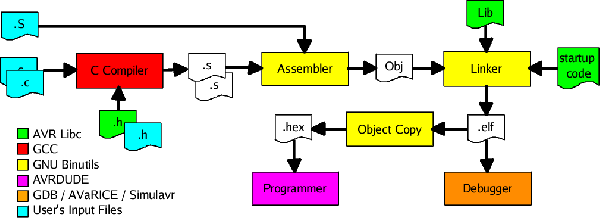
\includegraphics[scale=0.5]{images_not_compressed/compchain.png}
			\label{compchain}
			\caption{Cross compilation and compilation difference}
		\end{center}
	\end{figure}

	